\chapter{2019/2020 Semester 1 Exam}
\section{Q1 (Short Questions)}

\begin{enumerate}[label=(\alph*)]
\item Using a simple atomistic model, show that the theoretical cohesive strength of an ideal elastic solid is of the order of its Young’s modulus. Is this upper limit ever approached in real materials? Using the same model, also show that the cohesive strength may be written as
$$\sigma_c = \sqrt{\frac{E\gamma_s}{x_o}}$$
where $E$ is Young's modulus, $\gamma_s$ is the surface energy per unit area and $x_o$ is the equilibrium lattice spacing. Comment on the accuracy of your result. \hfill(10 marks)

\item Describe the energy balance approach to fracture as originally proposed by Griffith. Explain how Griffith used this approach to successfully predict the fracture strength of glass. Why does the direct application of Griffith's result grossly underestimate the fracture strength of metals? \\ \hfill(10 marks)

\item What is meant by the `plane strain fracture toughness of a material', $K_{Ic}$? When carrying out a standard laboratory test to determine $K_{Ic}$ for a given material, discuss the restrictions that apply to the dimensions of the test specimens in order to obtain a valid result. How are these restrictions overcome for tough materials in more recent standards such as ASTM E1820:2001? \hfill(10 marks)

\item What is meant by an `$R$-Curve' in the context of the fracture resistance characteristics of a material. Discuss the factors influencing the shape of the $R$-Curve, giving examples of materials exhibiting flat, rising and falling $R$-Curves and the underlying fracture mechanisms which cause this behaviour. \hfill(10 marks)


\item Briefly describe how linear elastic fracture mechanics may be used to characterize fatigue crack growth under constant amplitude cyclic loading conditions. Explain how the occurrence of variable amplitude loading influences the propagation of a fatigue crack. \hfill(10 marks)


\item Describe the typical variation of triaxiality in the vicinity of a mode I crack front and show how different levels of constraint in plane stress and plane strain lead to relatively large differences in the size and shape of the plastic zone under these conditions. \hfill(10 marks)

\item Briefly discuss the role of the $J$-integral in elastic-plastic fracture mechanics. In particular, describe how the $J$-integral may be viewed as both an energy parameter and a stress intensity parameter, and discuss the relationship between the $J$-integral and the other widely used elastic-plastic parameter, the crack tip opening displacement (CTOD). \hfill(10 marks)
\end{enumerate}
\hfill(Total: 70 marks)


\subsection{Q1 Solution}

\begin{enumerate}[label=(\alph*)]
    \item The potential energy-atomic separation relationship for a pair of atoms typically takes the following form:
    \begin{figure}[htb]
        \centering
        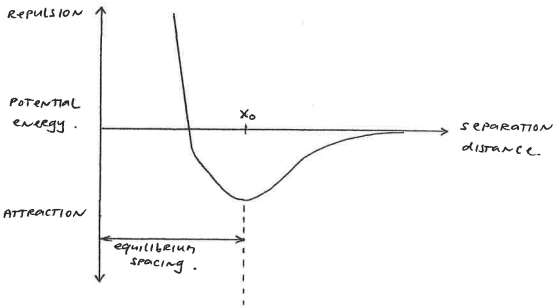
\includegraphics[width=0.8\linewidth]{exam./2019_atom_energy_sep.PNG}
        \caption{caption}
        %\label{fig:label}
    \end{figure}
    Where $x_0$ is the equilibrium spacing between two atoms.


    The force-separation relationship is as follows:
    \begin{figure}[htb]
        \centering
        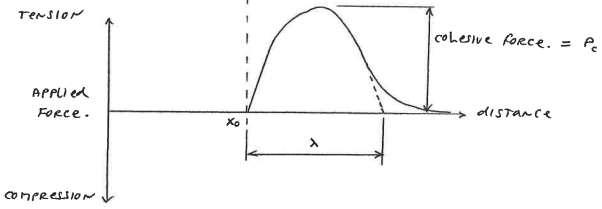
\includegraphics[width=0.8\linewidth]{exam./2019_atom-force-sep}
        \caption{caption}
        %\label{fig:label}
    \end{figure}
    Approximate the force-separation curve as half the period, $\lambda$, of a sine wave. Take origin at $x=x_0$, then we have:
    \begin{align}
        P&=P_c \sin^2\left(\frac{\pi x}{\lambda}\right)\\%\label{eq:label}
    \intertext{For small displacements, $\sin x \approx x$}
        \Rightarrow P&\simeq P_c \left(\frac{\pi x}{\lambda}\right)%\label{eq:label}
    \end{align}
    The bond stiffness is the slope of the force-displacement diagram
    \begin{equation}
        k = \frac Px = \frac{P_c \pi}{\lambda}%\label{eq:label}
    \end{equation}
    Relating this to the bulk properties of the material:
    \begin{equation}
        E = \frac{\sigma}{\varepsilon}\text{,}\;\;\;\; \sigma = \frac FA\text{,}\;\;\;\; \varepsilon=\frac{\text{displacement}}{\text{gauge length}}=\frac{x}{x_0}%\label{eq:label}
    \end{equation}
    




    \item fdsfa 
\end{enumerate}


